\chapter{Esquema TT. Protección diferencial}
\section{Análisis del esquema TT}
En este esquema están conectados a tierra tanto el centro de la estrella del transformador como las masas. Se produce un defecto fase-tierra con tierra de retorno.
\begin{figure}[H]
	\centering
	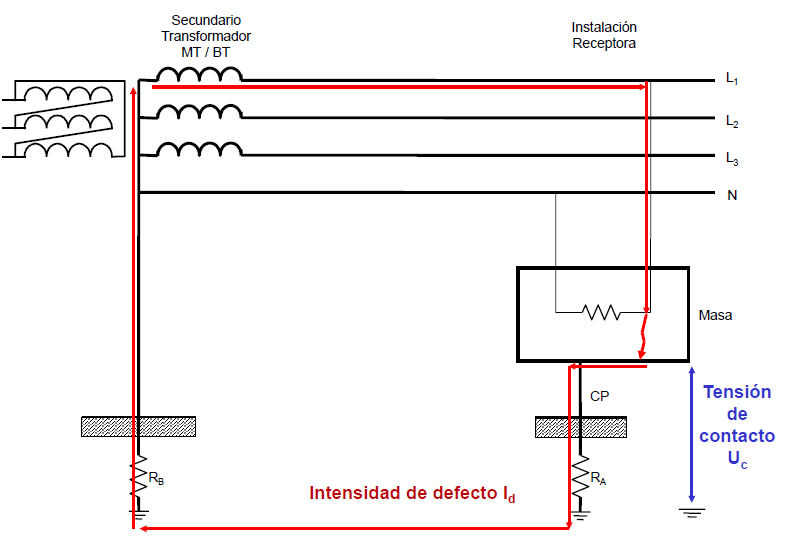
\includegraphics[width=0.5\linewidth]{Images/26}
	\label{fig:26}
\end{figure}

Su circuito equivalente es:
\begin{figure}[H]
	\centering
	\begin{adjustbox}{width=1\textwidth}
	
		\begin{circuitikz}
			\tikzstyle{every node}=[font=\normalsize]
			\draw (5.25,14.25) to[sinusoidal voltage source, sources/symbol/rotate=auto,l={ \normalsize $cU_{\text{fase-neutro}}$}] (5.25,11.25);
			\draw (6,15.5) to[european resistor,l={ \normalsize $\dfrac{2}{3} Z_{\text{media tension}}$}] (11,15.5);
			\draw (5.25,14.25) to[short] (5.25,15.5);
			\draw (5.25,15.5) to[short] (6.25,15.5);
			\draw (11,15.5) to[european resistor,l={ \normalsize $Z_{\text{trafo}}$}] (13.5,15.5);
			\draw (13.5,15.5) to[european resistor,l={ \normalsize $R_{\text{línea}}$}] (15.5,15.5);
			\draw (15.5,15.5) to[european resistor,l={ \normalsize $R_{\text{defecto}}$}] (15.5,12.75);
			\draw (15.5,12.75) to[european resistor,l={ \normalsize $R_{\text{cable protección}}$}] (15.5,10.75);
			\draw (15.5,10.75) to[european resistor,l={ \normalsize $R_{\text{puesta a tierra masas utilización}}$}] (15.5,8.5);
			\draw (5.25,11.25) to[european resistor,l={ \normalsize $R_{\text{puesta a tierra neutro}}$}] (5.25,8.5);
			\draw (5.25,8.5) to (5.25,8.25) node[ground]{};
			\draw (15.5,8.5) to (15.5,8.25) node[ground]{};
			\draw [ color={rgb,255:red,200; green,0; blue,255}, <->, >=Stealth] (14.25,13) -- (14.25,7.75)node[pos=0.5, fill=white]{$U_{contacto}$};
			\draw [ color={rgb,255:red,200; green,0; blue,255}, ->, >=Stealth] (8.5,14.75) -- (12.5,14.75)node[pos=0.5, fill=white]{$I_{defecto}$};
			\node [font=\normalsize, color={rgb,255:red,200; green,0; blue,255}] at (8.5,16.25) {$Z_{MT}$};
			\node [font=\normalsize, color={rgb,255:red,200; green,0; blue,255}] at (12.25,16.25) {$Z_T$};
			\node [font=\normalsize, color={rgb,255:red,200; green,0; blue,255}] at (14.5,16.25) {$R_F$};
			\node [font=\normalsize, color={rgb,255:red,200; green,0; blue,255}] at (16.5,14.5) {$R_d$};
			\node [font=\normalsize, color={rgb,255:red,200; green,0; blue,255}] at (16.5,12.25) {$R_{CP}$};
			\node [font=\normalsize, color={rgb,255:red,200; green,0; blue,255}] at (16.5,10) {$R_A$};
			\node [font=\normalsize, color={rgb,255:red,200; green,0; blue,255}] at (6.5,10.25) {$R_B$};
			\node [font=\normalsize, color={rgb,255:red,200; green,0; blue,255}] at (6.5,13.25) {$cU_0$};
		\end{circuitikz}
	\end{adjustbox}
	\label{fig:my_label}
\end{figure}

En estas condiciones:
\begin{equation}
	Z_{bucle}=\dfrac{2}{3}Z_{MT}+Z_T+Z_F+R_d+R_{CP}+R_A+R_B
\end{equation}
\begin{equation}
	I_d=\dfrac{c U_0}{Z_{bucle}}
\end{equation}
\begin{equation}
	U_c=\left(R_{CP}+R_A\right)I_d
\end{equation}
\subsection{Circuito equivalente simplificado en caso de fallo}
Normalmente las resistencias de puesta a tierra son mayores que el resto de impedancias:
\begin{equation}
	R_B+R'_A \ggg \dfrac{2}{3}Z_{MT}+Z_T+Z_F+R_d
\end{equation}

El caso más desfavorable desde el punto de vista de la protección:
\begin{equation}
	R_d=0
\end{equation}

La resistencia desde la masa de utilización a tierra:
\begin{equation}
	R_A'=R_A+R_{CP}
\end{equation}
\begin{center}
	\begin{figure}[H]
		\centering
	\begin{adjustbox}{width=0.5\textwidth}
		
		\begin{circuitikz}
			\tikzstyle{every node}=[font=\normalsize]
			\draw (5.25,14.25) to[sinusoidal voltage source, sources/symbol/rotate=auto,l={ \normalsize $cU_0$}] (5.25,11.25);
			\draw (5.25,14.25) to[short] (5.25,15.5);
			\draw (5.25,15.5) to[short] (6.25,15.5);
			\draw (15.5,10.75) to[european resistor] (15.5,8.5);
			\draw (5.25,11.25) to[european resistor] (5.25,8.5);
			\draw (5.25,8.5) to (5.25,8.25) node[ground]{};
			\draw (15.5,8.5) to (15.5,8.25) node[ground]{};
			\draw [ color={rgb,255:red,200; green,0; blue,255}, <->, >=Stealth] (14.25,10.75) -- (14.25,7.75)node[pos=0.5, fill=white]{$U_{contacto}$};
			\draw [ color={rgb,255:red,200; green,0; blue,255}, ->, >=Stealth] (8.5,14.75) -- (12.5,14.75)node[pos=0.5, fill=white]{$I_{defecto}$};
			\node [font=\normalsize, color={rgb,255:red,200; green,0; blue,255}] at (16.25,9.5) {$R'_A$};
			\node [font=\normalsize, color={rgb,255:red,200; green,0; blue,255}] at (6,10) {$R_B$};
			\draw (6.25,15.5) to[short] (15.5,15.5);
			\draw (15.5,10.75) to[short] (15.5,15.5);
		\end{circuitikz}
	\end{adjustbox}
	\label{fig:my_label}
\end{figure}
\end{center}

En estas condiciones:
\begin{equation}
	R_S=R_{CP}+R_A+R_B
\end{equation}
\begin{equation}
	I_d=\dfrac{c U_0}{R_S}
\end{equation}
\begin{equation}
	U_c=\left(R_{CP}+R_A\right)I_d
\end{equation}

\textbf{Se debe disparar en caso de defecto mediante un interruptor diferencial.}
\section{Condiciones de protección}
Se debe cumplir que el producto de la resistencia de la toma de tierra y los conductores de protección con la corriente de corte de protección sea menor a la tensión de contacto límite:
\begin{equation}
	R_A \cdot  I_{\Delta n} \le U_L
\end{equation}

La tensión limite de contacto es:
\begin{itemize}
	\item Local seco: 50V
	\item Local húmedo: 24V
	\item Local sumergido: 12V
\end{itemize}

Existe una tabla con los tiempos máximos de corte según la tensión de fase:
\begin{table}[H]
	\centering
	\begin{tabular}{|c|c|}
		\hline
		\textbf{Tensión nominal fase-tierra $U_0$ (V)} & \textbf{Tiempo de corte máximo c.a. (s)} \\ \hline
		$120 < U_0 \leq 230$ & 0,2 \\ \hline
		$230 < U_0 \leq 400$ & 0,07 \\ \hline
		$U_0 > 400$ & 0,04 \\ \hline
	\end{tabular}
	\label{tabla:tension_tiempo_corte}
\end{table}

Se pueden instalar interruptores diferenciales selectivos con tiempo máximo de disparo de 1 segundo.
\section{Interruptor diferencial}
Constructivamente es una bobina que amplifica la diferencia de corriente entre fases y neutro:
\begin{figure}[H]
	\centering
	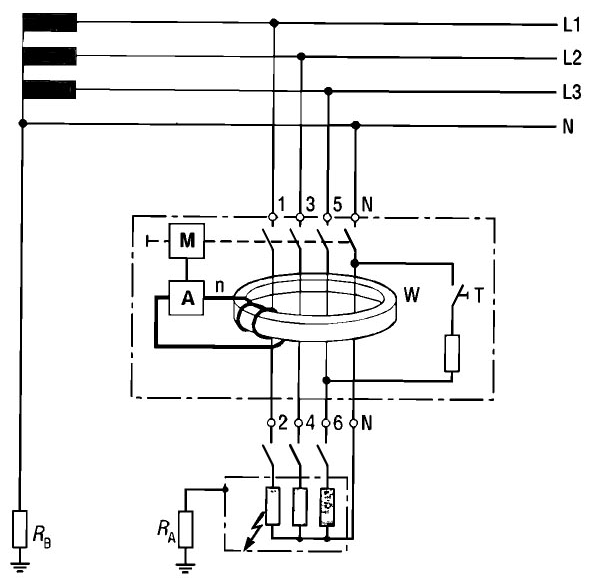
\includegraphics[width=0.7\linewidth]{Images/27}
	\label{fig:27}
\end{figure}

\subsection{Sensibilidad}
Se define el valor de sensibilidad, $\Delta In$, como el valor a partir del cual se asegura la apertura del interruptor diferencial. No obstante, puede producirse apertura a partir de la mitad de dicho valor.
\newline

Tipos de diferenciales según sensibilidad:
\begin{itemize}
	\item Alta sensibilidad: 6 – 10 – 30 mA
	\item Media sensibilidad: 100 – 300 – 500 mA
	\item Baja sensibilidad: 1 – 3 – 10 - 30 A
\end{itemize}

\subsection{Clase de dispositivos diferenciales según la corriente a detectar}
\begin{itemize}
	\item \textbf{Diferencial clase AC}: Detecta señales diferenciales senoidales de 50 Hz
	\item \textbf{Diferencial clase A}: Detecta señales senoidalesy pulsantes, en las dos polaridades
	\item \textbf{Diferencial clase F}: Detecta señales senoidalesy pulsantes de 50 Hz con componentes mezcladas de hasta 1000Hz
	\item \textbf{Diferencial clase B}: Detecta lo mismo que un clase F pero añadiendo señales de componente de corriente continua pura
\end{itemize}

Pueden estar inmunizados a altas frecuencias o a transitorios.

\subsection{Tiempo de funcionamiento}
En la siguiente tabla se recoge el tiempo de disparo de un interruptor diferencial en función de la relación intensidad de defecto, sensibilidad.

	\begin{figure} [H]
		\centering
		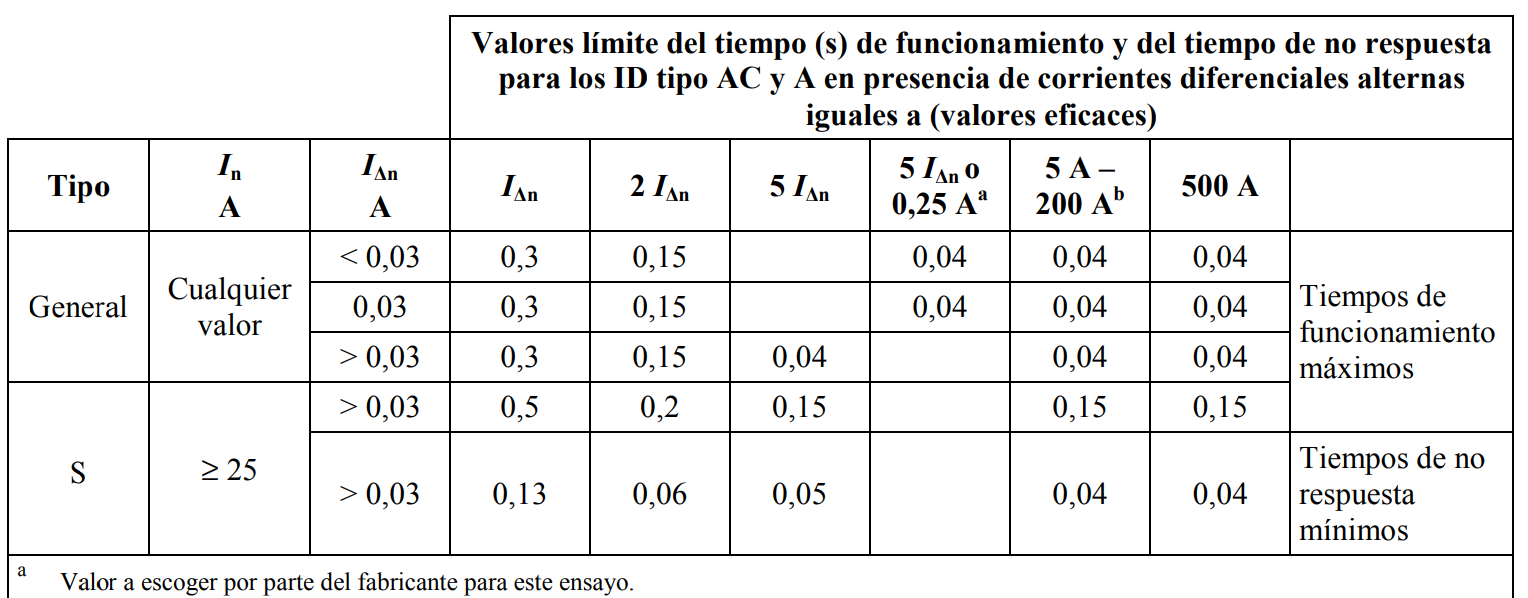
\includegraphics[width=0.7\linewidth]{Images/28}
		\label{fig:28}
	\end{figure}
	


\section{Selección de interruptores diferenciales}
\subsection{Intensidad asignada}
Para que el interruptor diferencial no sufra sobrecargas debe cumplirse que el diferencial no dispare antes que el interruptor automático.
\begin{equation}
	I_{n_{diff}}> I_{d_{auto}}
\end{equation}

Los fabricantes suministran tablas de asociación entre diferenciales e interruptores automáticos y entre diferenciales y fusibles
\subsection{Sensibilidad para protección}
Se calcula la intensidad de defecto, $I_d$, la tensión de contacto, $U_c$ y a partir de ello la sensibilidad:
\begin{equation}
	I_{\Delta n}\le \dfrac{U_L}{R_A}
\end{equation}

Además de esto, en algunas instalaciones se debe tener unas sensibilidad máximas concretas:
\begin{itemize}
	\item 10 mA:
	\begin{itemize}
		\item \textbf{Quirófanos}:Para los equipos no alimentados por transformador de aislamiento, sensibilidad
	\end{itemize}
	\item 30 mA:
	\begin{itemize}
		\item Viviendas
		\item Equipamiento eléctrico de bañeras con hidromasaje
		\item Tomas de corriente de intensidad asignada inferior a 20 A situadas a la intemperie y para proteger equipos portátiles para ser utilizados a la intemperie
		\item Ferias y stands:equipos eléctricos accesibles al público, circuitos de alumbrado y tomas de corriente
		\item Piscinas y fuentes:se admite en algunas zonas como medida de protección el corte automático por diferencial
	\end{itemize}
	\item 300 mA:
	\begin{itemize}
		\item Alumbrado exterior
	\end{itemize}
\end{itemize}
\subsection{Sensibilidad para evitar disparos intempestivos}
Se debe cumplir que no dispare con las corrientes de fuga:
\begin{equation}
	\sum I_{fuga} < \dfrac{I_{\Delta n}}{2}
\end{equation}

Se pueden originar corrientes de fuga por:
\begin{itemize}
	\item Efecto capacitivo del aislamiento de los cables de la instalación
	\item Armónicos
	\item Transitorios de corriente de muy poca duración
	\item Filtros capacitivos conectados a tierra de los equipos electrónicos
\end{itemize}

Para evitar disparos intempestivos se pueden tomar las siguientes medidas:
\begin{itemize}
	\item Limitar el número de tomas protegidas por un mismo diferencial
	\item Utilizar receptores de clase II
	\item Transformador de aislamiento en grupos de receptores muy contaminantes
	\item Menor sensibilidad del diferencial respetando las condiciones del RBT
	\item Uso de diferenciales inmunizados o temporizados
	\item Uso de diferenciales con función vigilante de aislamiento
	\item Uso del esquema TN-S
	\item Medidas para la instalación de núcleos toroidales separados para reducir el riesgo de desconexión intempestiva por corrientes de arranque importantes
\end{itemize}
\subsection{Tiempo de funcionamiento}
Se calcula:
\begin{equation}
	\dfrac{I_d}{I_{\Delta n}}
\end{equation}

Se obtienen los tiempos de funcionamiento según las tablas y se comprueba que son adecuados.
\section{Selectividad entre interruptores diferenciales}
El interruptor diferencial no limita corrientes de defecto, que suelen ser muy superiores a la sensibilidad. Como no es posible la selectividad amperimétrica se emplea selectividad cronométrica.
\section{Protección contra incendios}
Con corrientes de 300 mA se pueden provocar incendios. Se necesita una potencia mínima necesaria para provocar un incendio de entre 60 – 100 W.
\begin{itemize}
	\item En esquemas TT y TN se protege con diferenciales con sensibilidad menor o igual a los 300 mA
	\item En el esquema IT se debe proveer de dispositivos de control de aislamiento
	\item No se admiten conductores CPN
\end{itemize}
\section{Peligro no detección}
Si la resistencia de defecto, $R_d$, es alta el defecto no se detecta. No obstante, es más desfavorable la protección.